
% Chapter Template
\chapter{Conception} % Main chapter title

\label{Chapter2} % Change X to a consecutive number; for referencing this chapter elsewhere, use \ref{ChapterX}

\lhead{Chapitre 2. \emph{Conception}} % Change X to a consecutive number; this is for the header on each page - perhaps a shortened title

%----------------------------------------------------------------------------------------
%	SECTION 1
%----------------------------------------------------------------------------------------

\section{Introduction}

Nous présentons dans ce chapitre notre approche qui se base sur la méthode de segmentation dynamique. 
Nous décrirons cette méthode ou, plus précisément, nous nous intéresserons à son architecture de découpage que nous exploiterons dans notre algorithme.
Nous terminons avec des essais de quelques variantes.

\section{Vue global de notre approche}
La méthode LBP offre effectivement un excelent outil pour caractériser une texture. Cependant, son role s'arrête la. Pour pouvoir détecter efficacement les textures, il nous faudra appliquer un algorithme de ségmentation. Nous avons porté notre choix sur l'algorithme de segmentation dynamique [HAM et.al 13] qui forme une étape primordiale de notre travail de détection. Il se nome de la sorte car il se base sur des tailles de ségments variantes (nous expliquerons dans ce qui suit notre choix). \\

Cependant cette méthode ne permet que de chercher une unique texture qui est connue déjà à l'avance. Notre méthode présente alors une généralisation qui permet de segmenter l'image et détecter toutes ses textures, et ce, en ayant aucune information au préalable, à part l'image elle même.\\

Notre méthode a pour but de détecter chaque texture dans les différents endroits où elle est présente dans une image, sans affecter les surfaces qu'occupent les autres textures. On représente cette détection en coloriant avec une couleur unique les surfaces qui contiennent une même texture.\\

Nous fixons une taille d'échantillon "\textit{t}". Nous prendrons comme premier lieu un carré de cette taille au point (0px,0px) qui contient une première texture, et nous chercherons des ségments similaire. Nous colorions tous les ségments de la même couleur "\textit{C}". Ensuite, nous feront de même pour le prochain carré de taille "\textit{t}" non colorié.\\

Plusieurs résultats très satisfaisants ont pu être obtenus avec cette approche, et différentes variantes de notre méthode ont été appliqué.

%----------------------------------------------------------------------------------------
%	SECTION 2
%----------------------------------------------------------------------------------------

\section{Méthode de découpage}

\subsection{Définition}
\indent Une méthode de découpage est une opération visant à rassembler des pixels entre eux suivant des critères pré-définis. Dans notre cas, les critères de similitudes seront basés sur la ressemblance des textures, définie elle par les paramètres de la méthode LBP (I.4.B).\\

\subsection{Algorithme de découpage dynamique}
\indent L'algorithme sur lequel nous allons nous baser est décrit dans l'algorithme 1 [HAM et.al 13].
Nous nous basons sur celui-ci pour notre méthode de généralisation. Nous supprimons, le test de ressemblance à la texture de référence [Algorithme 1 - 4.c] pour sauvegarder tous les carrés générés.\\
\indent Nous supprimons cependant la phase de coloriage dans le test (6) [Algorithme 1 - 6] pour la remplacer par un \textit{return} qui nous retournera le tableau de tout les carrées sauvegardés.

Le processus de division est expliqué dans la figure suivante. [Figure 2.1]

\indent Nous avons choisi d'appliquer cet algorithme dans le but de proposer une solution de généralisation pour la recherche et la détection de plusieurs textures différentes qui sont présentes dans une image, car son aspect dynamique lui offre une bonne robustesse dont on peut citer :\\

\begin{itemize}
\item Des carrés de tailles différentes peuvent être extraits et analysés, grâce à leurs tailles dynamiques. L'ensemble comparé avec la fenêtre principale serait donc très riche et varié\\

\item Différentes formes hormis les carrés et différents points de convergence peuvent être considérés. Par conséquent, différentes configurations peuvent être étudiées.\\

\item L'indépendance entre l'architecture proposée et la méthode d'extraction des caractéristiques est le principal avantage de notre approche. Ce qui permet à cette méthode de s'adapter à différents cas d'utilisations.\\

\end{itemize}

%-------------- DEBUT : DECOUPAGE DYNAMIQUE -------------
\label{Algorithme de découpage dynamique}
\begin{algorithme}[H]
\caption{Algorithme de découpage dynamique}
\Function{Square dynamic decomposition system}
{\textit{img} : \textbf{image},\textit{textureRef} : \textbf{image}}{void}
{

1 Choose the converging point\textit{a}.\\
2  Consider the main window\\
3  Generate as many windows as possible(with the same size of MW)\\

4 \For { each window }
{
		\begin{itemize}
			\item[a] Apply the feature extraction method (LBP method);
			\item[b] Calculate the feature vector (LBP histogram);
			\item[c] Calculate the similarity Sim between the window’s feature with the sought texture feature
 			
		\end{itemize}\\

		d \If {\textit{Sim} is above the threshold}{ 
			Save the window’s position and its feature vector V
		}
}

5 Reduce the size of MW by the distance \textit{d}\\
6 \IfThenElse { the size of MW is below the minimum size }
	{
		Color the saved windows and terminate the process
	}
	{
		Goto step \textbf{3}
	}
}
\end{algorithme}

%-------------- FIN : DECOUPAGE DYNAMIQUE -------------

%----------------------------------------------------------------------------------------
%	SECTION 3
%----------------------------------------------------------------------------------------


\begin{figure}[H]
	\centering
		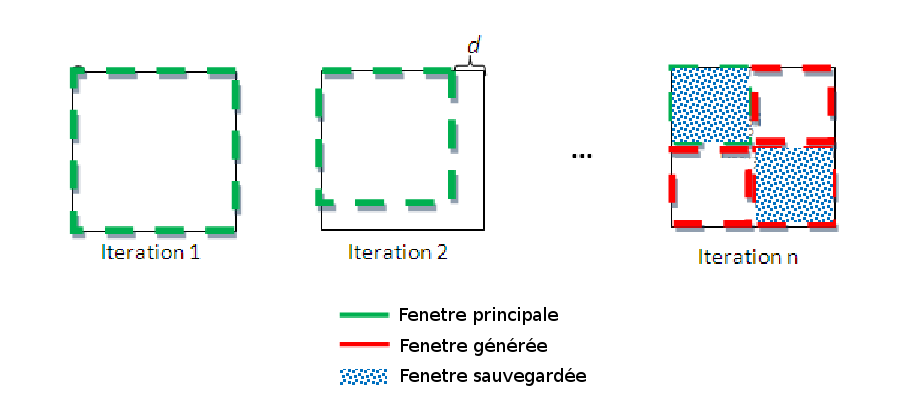
\includegraphics[width=14cm,]{Figures/chap2/1.png}
		
	\caption[division]{Processus de division.}
	\label{fig:division}
\end{figure}

\section{Généralisation de la méthode de recherches dynamique}

\indent Nous allons maintenant aborder tous les détails de notre approche de généralisation de la méthode cité ci-dessus.\\

\indent L'objectif étant de développer une méthode automatique de détection de toutes les textures présentes dans une image donnée, tout en minimisant au plus l'intervention de l'utilisateur. Chaque texture sera coloriée d'une couleur aléatoire et unique.

\subsection{Algorithme de généralisation}


%-------------- DEBUT : ALGORITHME DE GENERALISATION -------------
\label{Algorithme de généralisation}
\begin{algorithme}[H]
\caption{Generalization Algorithm}
\Function{Generalization Algorithm}
{\textit{img} : \textbf{image}}{void}
{
1 Constructing a blanc image with the same dimensions as \textit{img}\\
2 Applying the Square Dynamic Decomposition System without colouring \\
3 Save the result in a file\\
4 Set up a minimal size \textit{t} and a \textit{treshold}.\\
5 \While{ White window of dimension \textit{t} exists}
{
	a Brows the image from right to left, and from top to bottom, and extract the first white window
	\textit{Ref} with the dimension \textit{t} \\
	b Calculate the LBP histogram of \textit{Ref}\\
		
	c \For {each square}
		{
			calculate the resemblance \textit{Resmb} of the LBP histogram of the square with \textit{Ref}'s histogram

			\If{$Resmb > treshold$}{ 
				Colour the correspondent surface in the blanc image. 
				}
		}

}
}
\end{algorithme}

%-------------- FIN : ALGORITHME DE GENERALISATION -------------

\subsection{Interprétation de l'algorithme}

\indent Dans un premier lieu, nous nous contenterons d'appliquer l'algorithme sur des images simples.\\
Une image blanche \textit{IB} de même taille que l'image à découper est générée [Figure 2.2]. C'est cette première qui sera coloriée progressivement et rendu comme résultat finale de l'opération.

\begin{figure}[H]
	\centering
		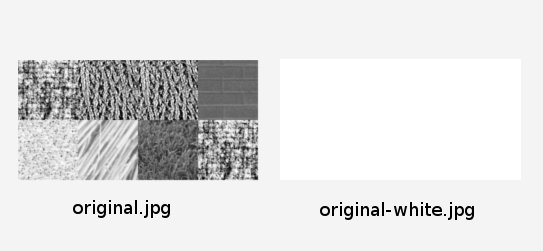
\includegraphics[width=14cm,]{Figures/chap2/2.png}
		
	\caption[initialisation]{Initialisation.}
	\label{fig:division}
\end{figure}

\indent L'algorithme de découpage présenté précédement est appliqué. Ce dernier nous retournera un ensemble de carrés que nous allons sauvegarder dans un fichier. La sauvegarde contiendra les coordonnées de l’extrémité initiale du carré (en haut à gauche) $(x_0,y_0)$ , sa taille \textit{t} et la valeur de son histogramme LBP \textit{h}. Le résultats sera un tableau  avec pour chaque carrée un élément : $elem = [x0,y0,t,h]$\\

\indent Ce qui nous permettra de ne plus avoir à refaire cette étape les prochaines fois qu'on traitera la même image.\\
\indent Nous fixons une taille $t_r$ pour les fenêtres de références que nous allons choisir à partir de l'image. Dans notre algorithme, nous l'avons fixé à \textit{30px}.\\
\indent Nous allons chercher une fenêtre vide de taille $t_r$. Cette dernière est représentée par un carré non encore colorié de la même taille et à la même position dans l'image blanche créée au début. Nous parcourons pour cela l'\textit{IB} de gauche à droite, et de haut en bas.\\
Si la fenêtre est trouvée, nous générons son histogramme LBP et la colorions d'une couleur \textit{C} (\textit{C}=marron, dans l'exemple ci dessous). [Figure 2.3]

\begin{figure}[H]
	\centering
		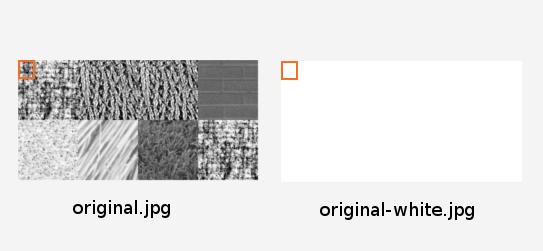
\includegraphics[width=14cm,]{Figures/chap2/3.png}
		
	\caption[detection1]{Première détection.}
	\label{fig:division}
\end{figure}

Nous allons parcourir les carrés créés par l'algorithme de découpage en comparant leurs histogrammes à celui de la référence détectée. \\

Il existe plusieurs méthodes pour calculer la distance entre deux histogrammes. Nous utilisons la méthode d'intersection défini comme  suit :\\

soit $h_1$ et $h_2$ les deux histogrammes à comparer. La valeur d de comparaison est égale à la somme des minimums des fréquences de $h_1$ et $h_2$ pour chacun de leurs éléments.
$$d(h_1,h_2)=\sum\limits_{i}\min(h_1(i),h_2(i)) $$
Plus les histogrammes se ressemblent, plus la valeur de d est grande. Son maximum vaut 1, si les histogrammes sont identiques.\\
Si la valeur de comparaison est au dessus du \textit{seuil}, le carré correspondant dans l'IB est colorié de la même couleur C. [Figure 2.4]\\

\begin{figure}[H]
	\centering
		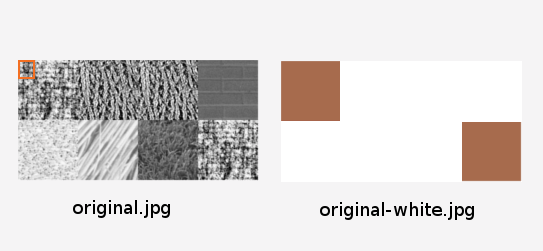
\includegraphics[width=14cm,]{Figures/chap2/4.png}
		
	\caption[coloriage1]{Coloration de la première texture détectée.}
	\label{fig:division}
\end{figure}

La recherche d'une nouvelle référence est entamée. On continu à chercher le premier carré blanc avec la même taille de références $t_r$ initialement fixée. [Figure 2.5]

\begin{figure}[H]
  \centering
    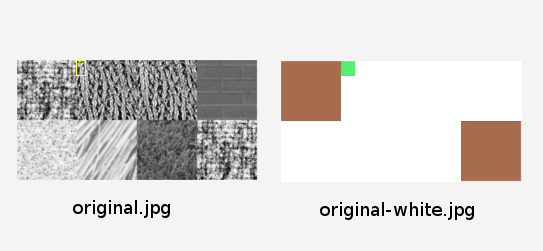
\includegraphics[width=14cm,]{Figures/chap2/5.png}
    
  \caption[detection2]{Deuxième détection.}
  \label{fig:division}
\end{figure}


Les carrés ressemblant à la nouvelle référence sont coloriés de la même façon. [Figure 2.6]

\begin{figure}[H]
  \centering
    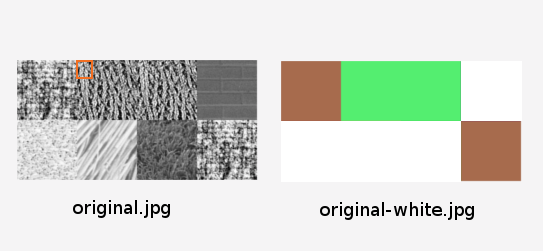
\includegraphics[width=14cm,]{Figures/chap2/6.png}
    
  \caption[coloriage2]{Coloration de la deuxième texture détectée.}
  \label{fig:division}
\end{figure}

Si aucun carré blanc de taille t ne reste dans l'IB, l'algorithme est terminé. [Figure 2.7]

\begin{figure}[H]
  \centering
    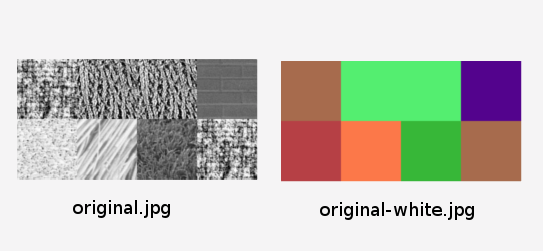
\includegraphics[width=14cm,]{Figures/chap2/7.png}
    
  \caption[coloriage]{Détection de toutes les téxtures.}
  \label{fig:division}
\end{figure}

\subsection{Variantes}
\indent Le premier problème à traiter pour une meilleure précision est de trouver le bon \textit{seuil} pour chaque texture recherchée. Et pour cela nous avons pensé à un algorithme d'apprentissage. Il s'agit d'une étape facultative. Cette dernière vise à tester d'une manière manuelle le meilleur \textit{seuil} possible pour une texture donné, et le sauvegarder dans une base de données.\\
\indent Quand vient l'étape de recherche de texture, les références seront recherchés dans la base de données suivant la ressemblance de l'histogramme sauvegardé et l'histogramme de la texture, et selon laquelle le meilleur \textit{seuil} sauvegardé sera extrait.

\subsubsection{LBP à rotation invariante }
\indent L'une des variante les plus intéressantes de la LBP est la $LBP^{riu2}$ qui est capable de détecter une texture même si cette dernière a subis une rotation d'un certain angle $\alpha$ qui est inclus dans l'ensemble suivant : $S = \lbrace 45\si{\degree}, 90\si{\degree}, 135\si{\degree}, 180\si{\degree}, 225\si{\degree}, 270\si{\degree}, 315\si{\degree} \rbrace$.\\

\indent Dans la figure 2.8, après que l'image ait subis une rotation de 45$\si{\degree}$, on remarque bien que le motif a aussi subit une rotation de 45$\si{\degree}$, mais le plus important est que le nouveau motif fait partie aussi des «\textit{uniform patterns}» tout comme le premier. 
Le motif a passé de la valeur $m=11000011$ vers la valeur $m'=11100001$.\\
De ce fait, on comprend qu'une rotation de l'image d'un angle de 45$\si{\degree}$ fait décaler les valeurs des motifs de un chiffre vers la droite, de manière générale on a :
$$ D = \frac{360\si{\degree}}{\alpha} $$
\indent La valeur du décalage $D$ dépend de la valeur de l'angle de rotation $\alpha$, et donc le choix de l'ensemble $S = \lbrace 45\si{\degree}, 90\si{\degree}, 135\si{\degree}, 180\si{\degree}, 225\si{\degree}, 270\si{\degree}, 315\si{\degree} \rbrace$ vient du fait que ce sont les seules valeurs de $\alpha$ qui donnent un nombre entier naturelle $D$ de décalage.


\begin{figure}[H]
	\centering
		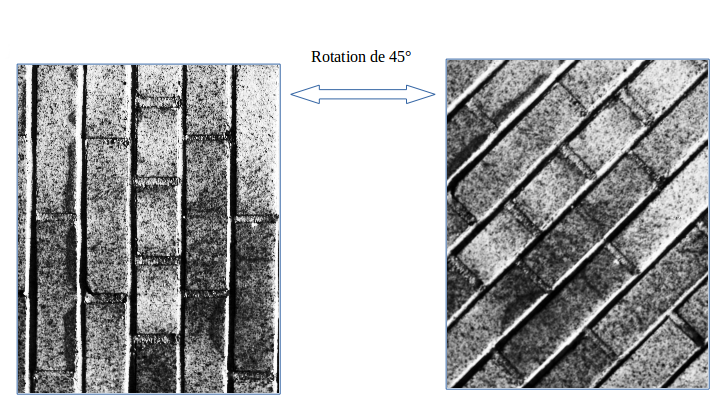
\includegraphics[width=14cm,height=8cm]{Figures/chap2/rotation45.png}
	\caption[rot1]{Un motif après une rotation de 45$\si{\degree}$}
\end{figure}


\indent Ainsi, comme chaque motif va subir un décalage de $D$ positions, et que les huit motifs résultants des huit décalages possibles, peuvent représenter toujours la même texture mais qui est sous des angles $\alpha$ différents, on peut donc regrouper les huit rotations possibles de chaque motif dans une seule valeur de l'histogramme comme le montre la figure 2.9.


\begin{figure}[H]
\centering
\begin{tabular}{cc}
\centering

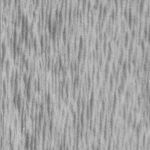
\includegraphics[width=5cm,height=4cm]{Figures/chap2/p4.png}
&
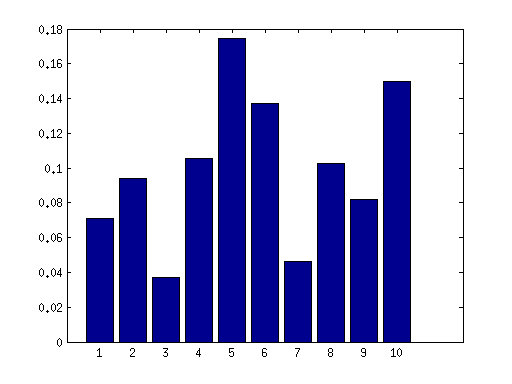
\includegraphics[width=9cm,height=4cm]{Figures/chap2/riu2a.png}\\

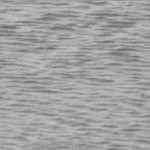
\includegraphics[width=5cm,height=4cm]{Figures/chap2/p5.png}
&
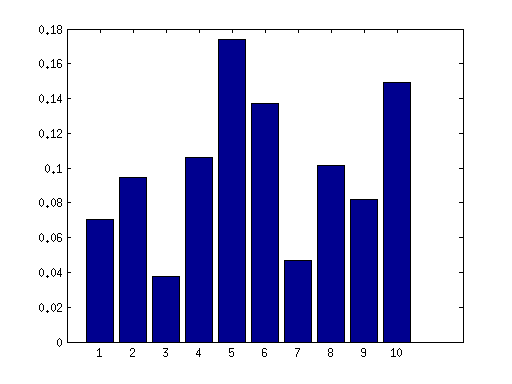
\includegraphics[width=9cm,height=4cm]{Figures/chap2/riu2b.png}\\
\end{tabular}
\caption[comp2]{Histogramme $LBP^{riu2}$ d'une texture subissant une rotation de 90$\si{\degree}$}
\end{figure}

\indent L'histogramme $LBP^{riu2}$ a dix valeurs différentes qui sont :
\begin{itemize}
\item Deux valeurs pour les motifs $m=00000000$ et $m=11111111$.
\item Sept valeurs pour les «\textit{uniform patterns}» uniques (incluant leur huit rotations) qui sont : $m=10000000$, $m=11000000$, $m=11100000$, $m=1111000$, $m=11111000$, \\
$m=11111100$, $m=11111110$.
\item Et une dernière valeur regroupant tous les «\textit{non uniform patterns}».\\
\end{itemize}

\indent On peut voir les meilleurs résultats obtenus dans la figure suivante :

\begin{figure}[H]
\centering
\begin{tabular}{cccc}
\centering

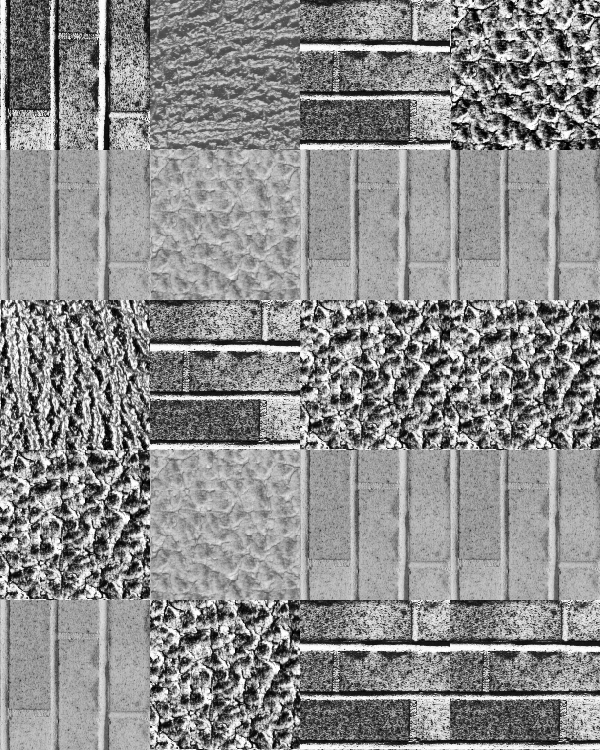
\includegraphics[width=4cm,height=4cm]{Figures/chap2/t1.png}
&

\includegraphics[width=4cm,height=4cm]{Figures/chap2/w1.png}
&
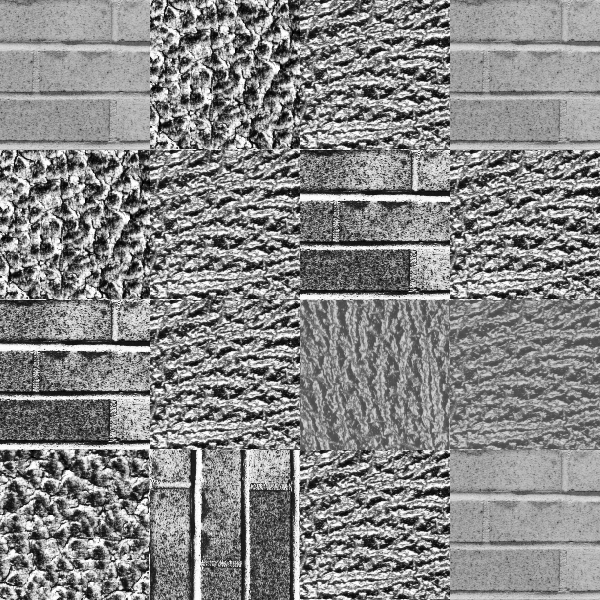
\includegraphics[width=4cm,height=4cm]{Figures/chap2/t2.png}
&

\includegraphics[width=4cm,height=4cm]{Figures/chap2/w2.png}
\end{tabular}
\caption[text3]{Segmentation avec la $LBP^{riu2}$}
\end{figure}

\indent Cependant dans certains cas, les résultats sont moins bons et cela revient au manque de précision de l'histogramme $LBP^{riu2}$, puisque chaque motif a été regroupé avec ses rotations, d'où résulte la difficulté du choix ... AJOUTER FIGURE HERE !!!!\\


\subsubsection{Segmentation par des formes circulaires}
\indent En plus de la recherche par des carrés, nous avons implémenté d'autres formes géométrique pour améliorer la détection de ces derniers.
Nous avons remarqué que, par exemple, les cercles n'étaient pas bien distingués par la méthode classique. \\
\indent Prenons l'image représentée dans la figure 2.8.

\begin{figure}[H]
	\centering
		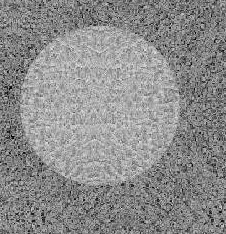
\includegraphics[width=7cm,]{Figures/chap2/8.png}
		
	\caption[img]{Image initiale.}
	\label{fig:division}
\end{figure}

La méthode classique nous a donné comme résultat l'image représenté par la figure 2.9.

\begin{figure}[H]
	\centering
		
\includegraphics[width=7cm,]{Figures/chap2/9.png}
		
	\caption[imgCarre]{Détection par carrés.}
	\label{fig:division}
\end{figure}

\indent Nous avons changé la détection et le coloriage des carrés par une détection et un coloriage en cercle.\\
Nous parcourons le cercle pour créer l'histogramme et le colorier à l'aide de la formule suivante:\\
\indent Prenons le centre $O(x_0,y_0)$ du cercle \textbf{c} d'un rayon \textbf{r}.  Un pixel $P (x_p,y_p)$ fait partie du cercle si l'inéquation ci-dessous est réalisée:
$$(x_p-x_0)^2 + (y_p-y_0)^2 <= R^2$$
Nous avons eu comme résultats l'image représentée par la figure 2.10.

\begin{figure}[H]
	\centering
		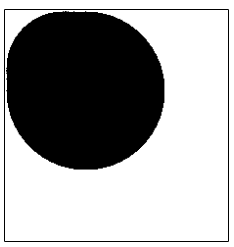
\includegraphics[width=7cm,]{Figures/chap2/10.png}
		
	\caption[imgCercle]{Détection par cercles.}
	\label{fig:division}
\end{figure}

%----------------------------------------------------------------------------------------
%	SECTION 4
%----------------------------------------------------------------------------------------

\section{Création des images de test}

\indent Les images sur lesquelles nous avons appliqué nos tests ont été généré aléatoirement. Les textures ont été tirés de la base de donnée \textit{Brodatz} [ref].

Nous avons utilisé un premier algorithme pour découper ces dernières en plus petite textures (de taille 150*150px) et les avons mis dans un dossier \textit{Textures}.

\label{algo decoupage}
\begin{algorithme}[H]
\caption{Cutting textures}
\Function{Textures' Cutting}
{\textit{Brodatz textures} : \textbf{folder}}{folder}
{
\For {Each image from \textit{Brodatz's textures}}
{
	\begin{itemize}
	\item Cut \textit{150x150} first pixels.
	\item Add the new texture to the \textit{Textures} folder
	\end{itemize}
}
\\
\Return \textit{Textures}
}
\end{algorithme}

Puis nous avons élaboré un algorithme qui sélectionne aléatoirement des textures à partir du dossier rempli précédemment et construit avec ces dernières une image à tester.

\label{algo creation}
\begin{algorithme}[H]
\caption{Création de l'image à traiter}
\Function{Create Test Image}
{\textit{Textures} : \textbf{folder}}{image}
{
Create a matrix \textit{M} of random dimensions
\For {each cell in \textit{M}}
{
	Affect a random texture from \textit{Textures}
}
\\
\textit{image} = transforming M into one image
\\
\Return \textit{image}
}
\end{algorithme}

\section{Conclusion}
\indent Nous avons présenté dans ce chapitre les détails de notre approche dans le but de segmenter les différents types de textures. Les techniques que nous avons utilisé et généralisé nous ont permis d'élaborer un programme qui détecte toutes les textures présentes sur une image quelconque, et cela d'une manière automatique.\\
\indent Les résultats des tests restent satisfaisante si nous respectons les contraintes cités au début de ce chapitre, et qui concernent la forme rectangulaire des textures recherchées. Nous avons aussi montré que d'autres formes de textures peuvent être appliquées à notre méthode afin de détecter des formes non rectangulaires.\\
\indent Nous présentons dans ce qui suit, notre application ainsi que des tests qui montreront les différents résultats obtenu à l'aide de cette méthode.
